\frame
{
  \frametitle{An approach using Piecewise Linear modeling}

}

 \frame
{
  \frametitle{Ideal Diode}
   \centerline{
  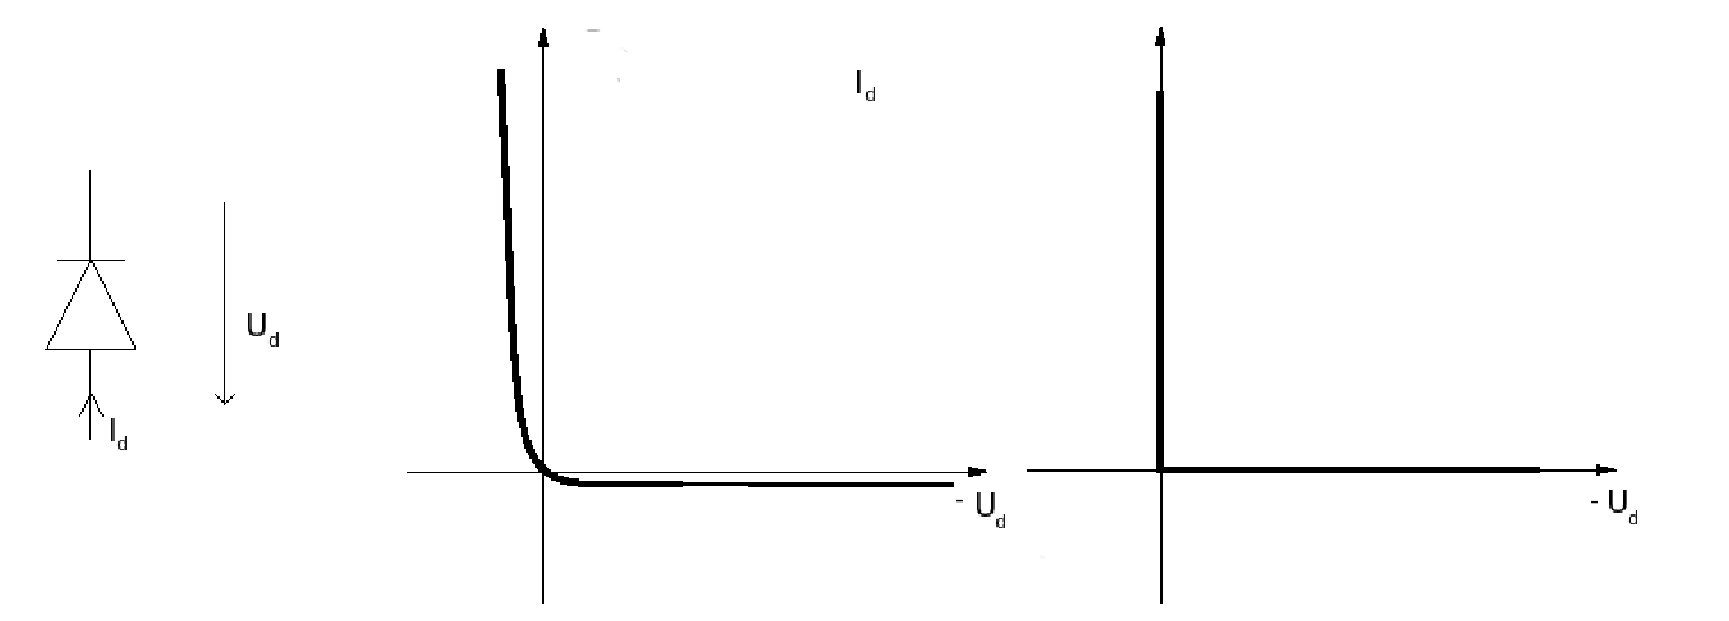
\includegraphics[width=100mm]{diode.eps}
  }
   \begin{block}{Branch Constitutive Equation of the diode:}
  \[ I_d =I_{s}(\exp{(-U_{D}/C)}-1)\]
  \end{block}
   \begin{block}{The complementary formulation:}
  \[0 \leq I_d \, \perp \, -U_{D} \geq 0\]
  \end{block}

}
\frame
{
  \frametitle{Ideal Transistor}
   \centerline{
  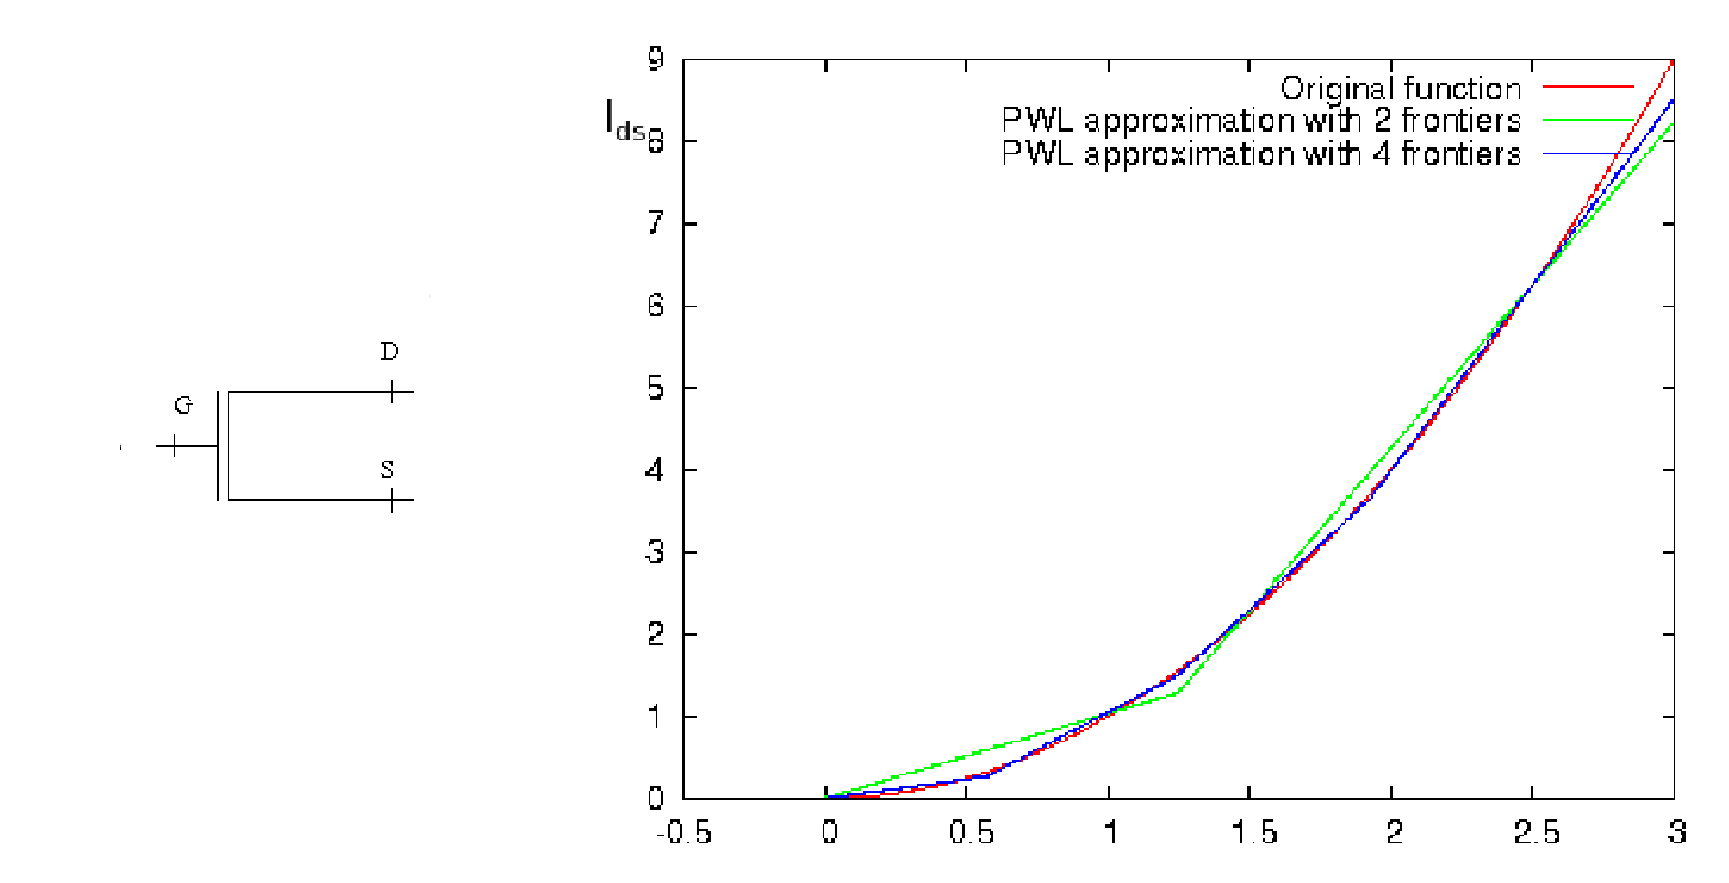
\includegraphics[width=100mm]{def2.eps}
  }
   \begin{block}{The complementary formulation:}
  \[ I_{d} = \left(\begin{array}{ccc}
  c_{1}&...&c_{10}\end{array}\right)\lambda \qquad  I_{d} = -I_{s}\]
  \[Y=A\left(\begin{array}{c}
  V_{d}\\
  V_{g}\\
  V_{s}\\\end{array}\right)+I\lambda + C\]
  \[0 \leq Y \, \perp \, \lambda \geq 0\]
  \end{block}

}
 
 \frame
{
\frametitle{Complementarity formulation.}

\begin{figure}
   \centerline{
   \scalebox{0.8}{
    \input{CSsmall.pstex_t}
    }
 } 
 \end{figure}

  
 \begin{eqnarray*}
 &{\color{Green}L\dot I_L -(V_1-V_2)=0}&V_3-e(t)=0\\
 &I_L-I_S-I_D=0&RI_L-V_2=0\\
 &{\color{Red}V_1+I_D(\lambda _4 +R_{on})}&{\color{Blue}V_1-20+I_S(\lambda _2 - R_{on})=0}\\
 &{\color{Red}y_3=R_{off}-\lambda _4 - R_{on}}&{\color{Blue}y_1=R_{off}-\lambda _2-R_{on}}\\
 &{\color{Red}y_4=-V_1+\lambda _3}&{\color{Blue}y_2=V_3-V_2+\lambda _1}\\
 \end{eqnarray*}
 \[0 \leq y_i \perp \lambda _i \geq 0\]
 }

\frame
{

\frametitle{Complementarity formulation.}
 \begin{figure}
 \input{CS}  
 \end{figure}

 }
